\documentclass[border=10pt]{standalone}
\usepackage[svgnames]{xcolor}
\usepackage{amsmath}
\usepackage{pgfplots}
\pgfplotsset{compat=newest}
\usepackage[sfdefault]{FiraSans}
\usepackage{FiraMono}
\renewcommand*\familydefault{\sfdefault}
\begin{document}
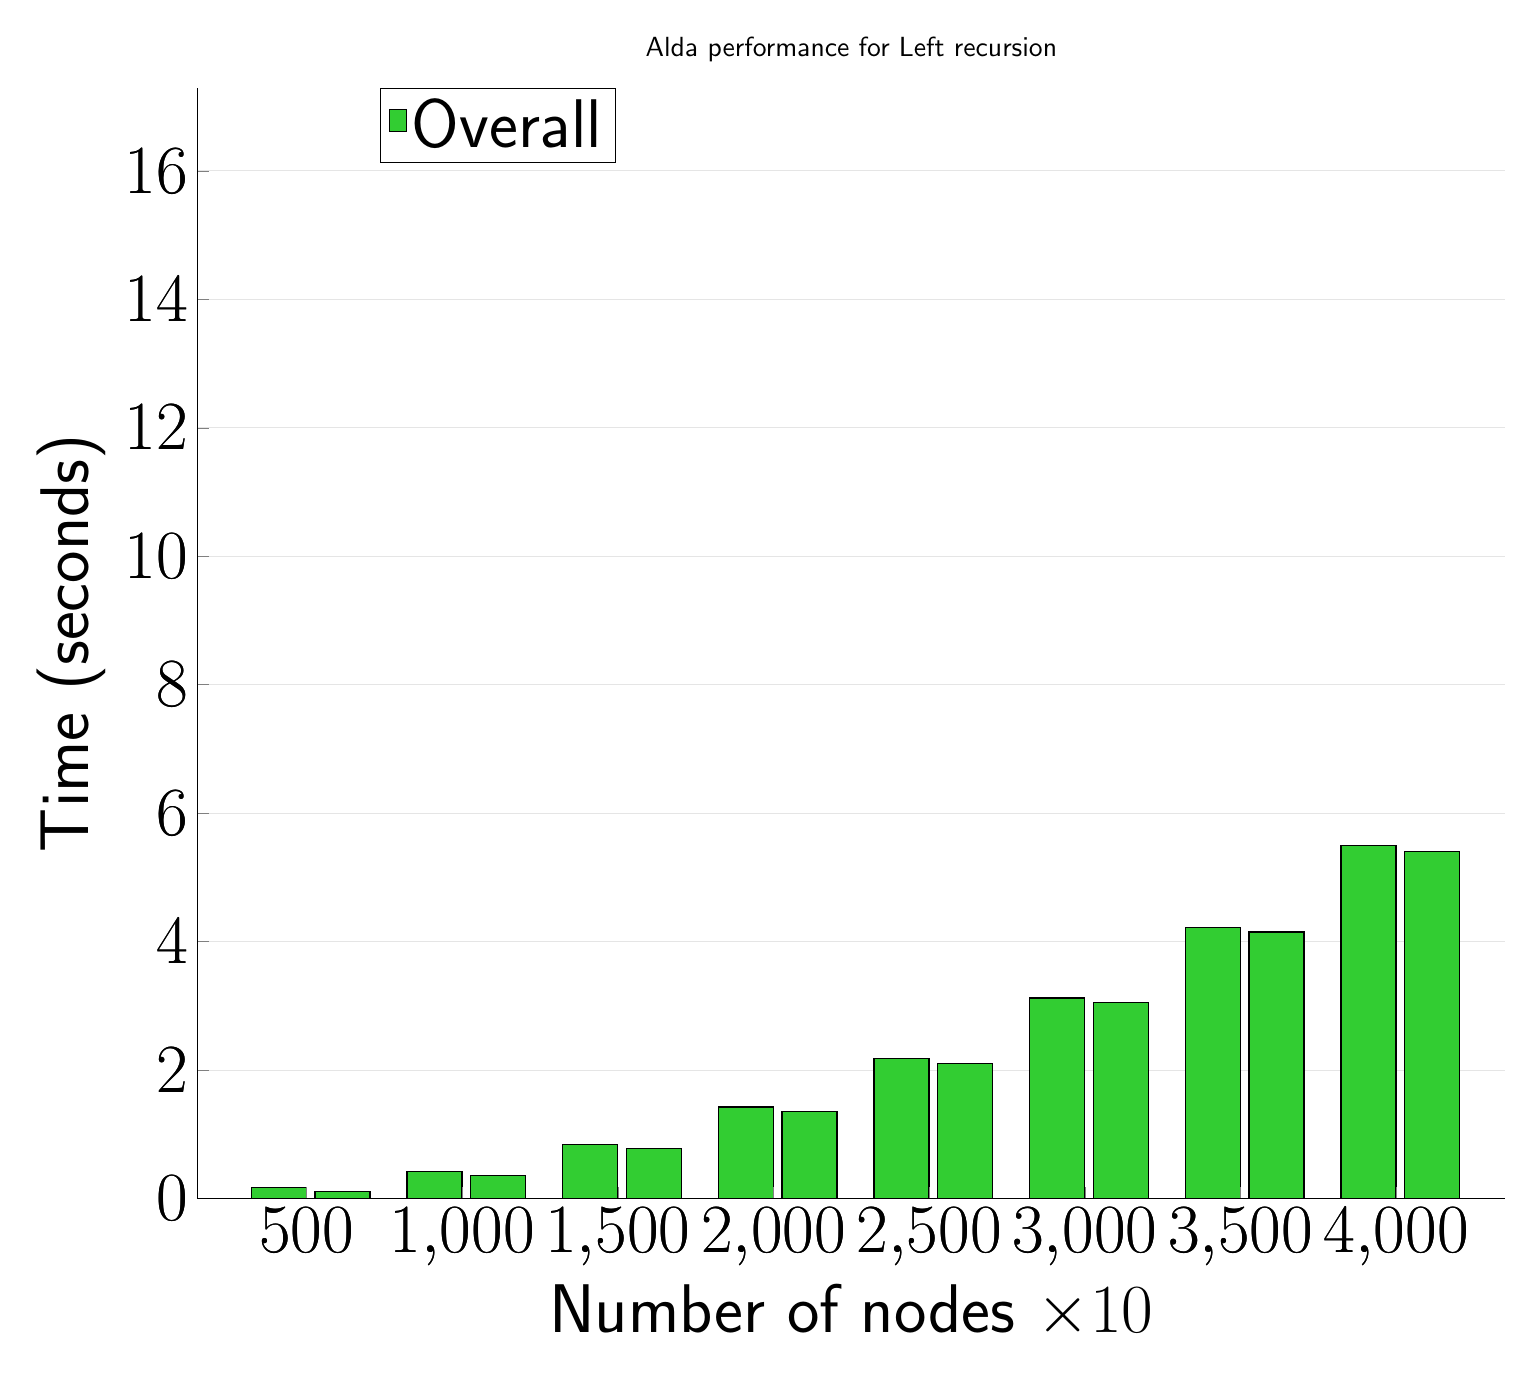
\begin{tikzpicture}
\begin{axis}[
   ybar stacked,
   title={Alda performance for Left recursion},
   bar shift=-10pt,
   width=1.5\textwidth,
   bar width=0.7cm,
   ymajorgrids, tick align=inside,
   major grid style={draw=gray!20},
   xtick=data,
   ymin=0, ymax=17.291999959945677,
   axis x line*=bottom,
   axis y line*=left,
   enlarge x limits=0.1,
   legend style={
       at={(0.23, 1)},
       anchor=north,
       legend columns=1,
       font=\Huge,
   },
   ylabel={Time (seconds)},
   xlabel={Number of nodes $\times 10$},
   label style={font=\Huge},
   tick label style={font=\Huge},
]
\addlegendimage{fill=LimeGreen, draw=black, line width=0.2pt}
\addlegendentry{Overall}
\addplot +[fill=LimeGreen, draw=black, line width=0.5pt] coordinates {
    (500, 0.1679999828338623)
    (1000, 0.41700000762939454)
    (1500, 0.8419999837875366)
    (2000, 1.4240000009536744)
    (2500, 2.1769999742507933)
    (3000, 3.122000050544739)
    (3500, 4.215999984741211)
    (4000, 5.495999979972839)
};
\end{axis}
\begin{axis}[
   ybar stacked,
   bar shift=13pt,
   width=1.5\textwidth,
   bar width=0.7cm,
   ymajorgrids, tick align=inside,
   major grid style={draw=none},
   xtick=data,
   ymin=0, ymax=17.291999959945677,
   axis x line*=none,
   axis y line*=none,
   enlarge x limits=0.1,
   label style={font=\Huge},
   tick label style={font=\Huge},
]
\addplot +[fill=LimeGreen, draw=black, line width=0.5pt] coordinates {
    (500, 0.10900000000000001)
    (1000, 0.35600000000000004)
    (1500, 0.7769999999999999)
    (2000, 1.3599999999999997)
    (2500, 2.1059999999999994)
    (3000, 3.053)
    (3500, 4.148)
    (4000, 5.405)
};
\end{axis}
\end{tikzpicture}

\end{document}
